%%%%%%%%%%%%%%%%%%%%%%%%%%%%%%%%%%%%%%%%%%%%%%%%%%%%%%%%%%%%%%%%%%%
%Conc_Ventilateur.tex : Projet de conception - Contrôle Arduino d'un Ventilateur | Électronique et mesures expérimentales GPH-2006, Physique électronique PHY-2002 | Département de physique, de génie physique et d'optique - FSG - Université Laval
%------------------------------------------------------------------
%Créé par Jérémie Guilbert, Louis-Philippe Dallaire,  & Marc-André Vigneault
%Contributions par Claudine Nì. Allen
%Compilateur pdfLaTeX, distribution TeX Live 2020
%Dernière modification CA : 23 novembre 2021
%
%ToDo
% - J'ai beaucoup de commentaires à l'intérieur du texte ci-dessous, tout relire et modifier selon comment ça va dans l'adaptation au mode hybride de retour post-pandémie.
%
% - Développer un/des compléments séparés (éliminer l'annexe éventuellement) et/ou capsules vidéo à pour les outils des ateliers et ce projet: Arduino (la carte et le IDE), Fritzing, Tinkercad, Falstad(possiblement bien avant dans les cours asynchrones avec ce dernier). Mentionner seulement dans la section logiciel du site de cours (pas matériel didactique obligatoire) et aborder plus au cours 6 présentiel qui traite entre autres de la 2e partie de la session.
%
% - Voir pour tourner le début du document en titre ou first-page only header et inclure un logo ULaval (si ok avec comms) : https://tex.stackexchange.com/questions/238520/how-to-correctly-include-a-header-image-only-on-the-first-page
% - Not sure I want this anymore... I'd like to reduce the bottom margin on the last page, I was fiddling with something like \AtEndDocument{\newgeometry{bmargin=0cm}}, but it doesn't work so far. See docs of fancyhdr package. Or try to work with "\thispagestyle{}" below the footer. 
%%%%%%%%%%%%%%%%%%%%%%%%%%%%%%%%%%%%%%%%%%%%%%%%%%%%%%%%%%%%%%%%%%%%

\RequirePackage[l2tabu, orthodox]{nag} %%Check for obsolete commands
\documentclass[english,french,12pt]{article}
%
%----------------------------------------------------------------
%### Loading Packages ###
%
%## Encoding, Typography & Language ##
\usepackage[utf8]{inputenc}
\usepackage[T1]{fontenc}
\usepackage{babel} %%is globally set to French, switch to English by inverting order in the '\documentclass' options
\usepackage{lmodern,csquotes} %%extended support for proper typesetting of accented letters & quotes with '\textquote{}' and the '\begin{displayquote}...\end{displayquote}' environment
\PassOptionsToPackage{mathscr}{eucal}\usepackage{amsfonts,eucal,mathrsfs,textcomp} %%math fonts and more symbols, extensively listed in the 'latex-AllSymbolList.pdf' of the 'Templates_labOMC' repo
\usepackage{ulem} %%underlining with '\uline{}', '\uwave{}' etc. and strikeout with '\sout{}'
\normalem
%\usepackage{newtxtext} %%for a Times New Roman text font output.

%## Colors, Boxes & Figures ##
\usepackage[usenames,x11names,table]{xcolor} %%colour names in 'xcolor-palettes.pdf' of the 'Templates_labOMC' repo. For printing, the [cmyk,dvipsnames] colour model is preferred.
%\usepackage{fancybox} %%more framed boxes
%\usepackage[breakable]{tcolorbox} %%coloured boxes with optional title
%\usepackage{float} %%more control on any floating environments 
%\usepackage{array,dcolumn,tabularx,multirow,longtable,booktabs} %%more control of 'tabular' and 'array' environments
\usepackage{graphicx,wrapfig,caption,sidecap} %%compiling with 'pdfLaTeX' supports .pdf,.pdf_tex .png, .jpg and .eps(indirectly) files. %Use '\includeinkscape' for .pdf_tex files exported from Inkscape or convert directly to TiKZ code with the 'svg2tikz' extension.

%## Maths & Physics ##
\usepackage{amsmath,amsthm,amssymb}
%\usepackage{cancel,trfsigns} %%math simplifications & signs for transforms respectively
%\usepackage[all]{xy} %%nice math diagrams
\usepackage{siunitx} %scientific & complex numbers, measurement & uncertainty, see 'latex-SIunitx.pdf' in the 'Templates_labOMC' repo.
\usepackage{physics} %typesetting for mathematical physics, see 'latex-PhysicsPack.pdf' in the 'Templates_labOMC' repo.
\usepackage{pgfplots} %graphs of symbolic functions and equations
%\usepackage{tikz-network} %%crystal lattice & complex networks drawing
%\usepackage{tikz-optics} %%optical drawing
%\usepackage{pstricks,pst-optexp,pst-optic} %%neat PSTricks optical drawing
%\usepackage{tikzorbital,chemfig,chemmacros,mhchem} %%chemical drawings/diagrams and formulae & safety
%\usepackage{pstricks,pst-labo} %%laboratory chemical glassware
%\usepackage{pstricks,dsptricks,pst-sigsys} %%signal processing plots/drawings
%\usepackage[RPvoltages,americanvoltages,americancurrents]{circuitikz} %%electrical circuit drawing with Rising Potential voltages
%\usetikzlibrary{babel} %%needed for electrical circuit drawing when running babel-french
%\usepackage{yquant} %%quantum circuit drawing

%## Miscellaneous Nice Tools ##
\usepackage{ccicons} %%Creative Commons icons, reusable content at <https://search.creativecommons.org/>
%\usepackage{media9,animate,tikz} %%tools for multimedia and general drawing
%\usepackage{pythontex} %%runs Python code in the LaTeX source files and typeset the output

%## Bibliography ##
%\usepackage[backend=biber,sorting=none]{biblatex} %%see 'cheatsheet-BibLaTeX.tex' in the 'Templates_labOMC' repo.
%\addbibresource{} %%import your .bib file in BibLaTeX format from Zotero

%## Hyperlinks ##
\usepackage{hyperref,xurl} %%'\href{_URL_}{_hypertext_}' to link the hypertext & '\url{_URL_}' to link the displayed web address, each internal '~\ref{_label_}' is also hyperlinked ; xurl for more line breaks.
\usepackage{doi} %%automatically resolves object identifiers such as IDs from doi, arXiv, OCLC, etc., use '\doi{}' if the former bugs.

%## Layout ##
%%Watch for conflicts with the overall document class.
\usepackage{geometry} %%page layout
\usepackage{fancyhdr}
\usepackage{setspace} %%interline spacing tools ; unit relative to current font: em ~width of an 'M' (uppercase), typically equal to the font size in pt
\usepackage{enumitem} %%tools to change list format
\usepackage{import}
%\usepackage{tasks,xsim,epigraph,boxedminipage,multicol,lscape,rotating,makeidx,showidx,glossaries}

%---------------------------------------------------------
%### Settings ###
%
%## Configuring the layout and other format setups ##
%\the\parindent{} , \the\value{equation} %%and other '\the' commands to see the current parameter, counter,... value
\geometry{  %%for geometry package
%    showframe,  %%uncomment to see lines delimiting the dimension boxes
    letterpaper,
    margin=0.75in}
\pagestyle{fancy}
\fancyhf{}
\renewcommand{\headrulewidth}{0pt}
\fancyfoot[C]{-\thepage-} %%bottom center page numbering
%\interfootnotelinepenalty=10000 %%uncomment if long footnotes are incorrectly spreading on several pages
\widowpenalty=300 %%increase for less likely widow lines
\clubpenalty=300  %%increase for less likely orphan lines
\setlength{\parskip}{1em plus0.4em minus0.2em} %%changing space between paragraphs
%\setlength\parindent{3em} %%uncomment to force indentation of all paragraphs or remove completely with 0em
%\setlist[enumerate]{wide=0pt,widest=99,leftmargin=\parindent,labelsep=*} %%Global changes of the [enumerate] list
\setcounter{equation}{0} %%ensure resetting of the equation counter
\captionsetup{  %%for figure and table captions
    font=footnotesize,
    labelfont=bf,
    labelsep=period,
    margin=5em}
    
%## Global settings for packages ##
\sisetup{separate-uncertainty=true} %%for SIunitx package
\hypersetup{   %%for hyperref package
    breaklinks=true,
    linktocpage=true,
    colorlinks=true,
    urlcolor=blue,
    linkcolor=blue,
    citecolor=blue,
    filecolor=blue}
\pgfplotsset{compat=1.9,width=5cm} %%for pgfplots package, backwards compatibility with 'compat'
\usetikzlibrary{arrows} %%for PGF/TikZ

%---------------------------------------------------------
%### Defining command shortcuts & macros ###
%
\newcommand{\be}{\begin{equation}} %%for numbered equations, use instead \[...\] to display without numbering or $...$ to include directly inline.
\newcommand{\ee}{\end{equation}}
\newcommand{\bea}{\begin{align}} %%number each equation and align them on &= the equal sign and more generally on the ampersand & character. 
\newcommand{\eea}{\end{align}}
\newenvironment{eqsplit}{\equation\aligned}{\endaligned\endequation}
\newcommand{\bes}{\begin{eqsplit}} %%defined the same way as the align environment, but considered as one equation on multiple lines with one number overall.
\newcommand{\ees}{\end{eqsplit}}
\newcommand{\beg}{\begin{gather}} %%gathering equations one below another without aligning.
\newcommand{\eeg}{\end{gather}}
\DeclareMathOperator{\TLs}{\mathscr{L}} %%Laplace transform symbol \TLs
\newcommand{\TLd}[1]{\TLs\!\left[#1\right]} %%Laplace transform operator \TLd{}
\DeclareMathOperator{\TLsi}{\mathscr{L}^{-1}} %%inverse Laplace transform symbol \TLsi
\newcommand{\TLi}[1]{\TLsi\!\left[#1\right]} %%inverse Laplace transform operator \TLi{}
\DeclareMathOperator{\TFsi}{\mathscr{F}^{-1}} %%inverse Fourier transform \TFsi
\newcommand{\TFi}[1]{\TFsi\!\left[#1\right]} %%inverse Fourier transform operator \TFi{}
\DeclareMathOperator{\TFs}{\mathscr{F}} %%Fourier transform \TFs
\newcommand{\TFd}[1]{\TFs\!\left[#1\right]} %%Fourier transform operator \TFd{}
\renewcommand*{\Re}{\mathop{}\!\mathfrak{Re}} %%Real part \Re redefined with 2 characters fraktur typesetting
\renewcommand*{\Im}{\mathop{}\!\mathfrak{Im}} %%Imaginary part \Im redefined with 2 characters fraktur typesetting

%---------------------------------------------------------
%### Titre triché pour mettre les auteurs en note de bas de page! ###
%
\title{\vspace{-7em}\thanks{Auteurs: Louis-Philippe Dallaire, Jérémie Guilbert, Marc-André Vigneault \& Claudine Allen}}
\date{}
\renewcommand\footnotemark{}

%---------------------------------------------------------
\begin{document}
%---------------------------------------------------------
\maketitle\thispagestyle{fancy}
%---------------------------------------------------------
%
%------ BEGIN HOMEMADE TITLE ------%
%inspiré de l'équipe du Prof. L.J. Dubé
%
\begin{center}
    \textbf{\large{Électronique et mesures expérimentales / Physique électronique}}\\
    \vspace{0.2em}
    \textbf{GPH-2006 / PHY-2002}

    \textsc{Département de Physique, de Génie Physique et d'Optique\\
    Faculté des Sciences et de Génie, Université Laval}
\end{center}

\vspace{-1em}
\noindent Automne 2021 \hfill Responsable: C. Allen\par
\vspace{0.2em}
\hrule
\vspace{0.5em}
\centering
    \textsc{Projet de Conception\\
    Contrôle Arduino d'un Ventilateur}\\
\vspace{0.5em}
{Dépôt sur Gradescope: 6 décembre \hfill Présentations: 7 décembre (voir horaire)}\par
\vspace{0.4em}
\hrule
\justify
%------ END HOMEMADE TITLE ------%

Pour progresser vers l'objectif d'autonomie et d'initiative nécessaire au travail de recherche, de développement et d'ingénierie, la dernière activité du cours ne donne aucun protocole ni schéma de circuit. Vous devez concevoir par vous-même le circuit qui répondra aux besoins à identifier dans la problématique ci-dessous et préparer les éléments demandés dans la section \nameref{subsec:livrables}. Pour ce faire, vous devrez faire appel aux ressources étudiées dans l'ensemble du cours et au-delà, notamment vous initiant au monde des microcontrôleurs à l'interface entre l'électronique et l'informatique. \textcolor{red}{En plus des informations en \nameref{sec:annexe} et en provenance des manufacturiers (fiches techniques), ...}

%culture maker, Do it yourself (DIY) communauté DIY, médigraphie, toute autre source, entraide TEAMS
\vspace{-1em}
\subsection*{Problématique}
\vspace{-0.5em}
L’été dernier, votre ami Itof Mèyacho a vécu la pire canicule de toute sa vie. En effet, comme il est étudiant, il ne peut se permettre d’avoir l’air conditionné tant convoité. Il doit se contenter d’un bon vieux ventilateur. Il souhaiterait trouver un moyen pour ajuster la vitesse de son ventilateur selon la luminosité du soleil qui entre dans son appartement, et ce, sans avoir à se lever de son sofa. Ses jeux vidéo ne peuvent attendre! De plus, bien qu’il fasse complètement noir dans sa chambre la nuit, il trouve essentiel que le ventilateur continue de tourner, mais à moindre vitesse, car le bruit du plein régime l’empêche de se reposer. Comme la prochaine canicule est à venir et qu’il semble trop occupé à jouer aux jeux vidéo, Itof Mèyacho vous demande votre aide. À l'aide de vos nouvelles connaissances en électronique, il est maintenant temps de lui donner un coup de main.

Après un peu de recherche et expérimentation, vous avez réussi à déterminer que le moteur du ventilateur d’Itof fonctionne en courant continu (DC en anglais). Vous avez aussi remarqué que le moteur ne peut pas tourner à une vitesse supérieure à 437~RPM sans risquer de se briser. Après quelques tests, Itof a identifié qu’il était confortable la nuit seulement lorsque le ventilateur tourne à une vitesse de 200~RPM. Vous décidez donc de concevoir un système basé sur un microcontrôleur Arduino. Celui-ci sera utilisé pour lire la luminosité ambiante à partir d’une photorésistance et ensuite ajuster la vitesse de rotation du moteur DC en fonction de la luminosité mesurée. En plein jour, quand la luminosité est maximale, le moteur doit fonctionner près de sa vitesse maximale de 437~RPM. Si la luminosité diminue, la vitesse du moteur doit ralentir en conséquence jusqu’à atteindre la valeur attendue en pleine nuit. Entre les deux valeurs de luminosité extrêmes, la vitesse du moteur doit pouvoir prendre le plus de valeurs possibles. Notez finalement qu'avant de procéder à l’assemblage de votre système en pratique, vous allez simuler et tester virtuellement son fonctionnement pour réduire les essais-erreurs, le débogage et la frustration(!) au laboratoire.
\vspace{-1em}

\subsection*{\color{red}Composants électroniques permis} 
\begin{itemize}
%%%VÉRIFIER VS MATÉRIEL COFFRE ET AJOUTER CE QUI MANQUE AVEC FRANÇOIS. CHECK NPN AVEC FICHE TECHNIQUE TRANSISTOR.
    \item Batteries \SI{9}{\volt}
    \item Carte \href{https://www.arduino.cc/en/Guide/ArduinoUno}{Arduino UNO} dont le fonctionnement est abordé en \nameref{sec:annexe}
    \item Amplis-ops~U741
    \item Transistors bipolaires NPN
    \item Moteur DC
    \item Des résistances \SIlist[list-final-separator = {, }]{12;33;270;560}{\ohm}, \SIlist[list-final-separator = {, }]{1;1.2;10; 18;100}{\kilo\ohm} et \SI{1}{\mega\ohm}
    \item Des condensateurs de \SI{100}{\nano\farad}
    \item Une photorésistance, aussi connue sous le nom de \textit{light-dependent resistor (LDR)} ou \textit{photocell} en anglais (NE PAS confondre avec une cellule solaire).
\end{itemize}
\vspace{-1em}

\subsection*{Contraintes supplémentaires}
\begin{enumerate}
    \item Vous pouvez utiliser autant de composants que nécessaires dans la liste ci-dessus. Toutefois, vous n’avez pas le droit d’utiliser des composants qui ne figurent pas dans cette liste.
    \item Vous devez viser un minimum de composants dans le circuit. %Difficile à évaluer, déterminer éventuellement un nombre maximum de composants à ne pas dépasser.
    \item Vous devez découpler l’impédance du circuit de la photorésistance de l’impédance du circuit ADC (convertisseur analogique-numérique) de l’Arduino à l'aide d'un suiveur de tension qui agit alors comme un tampon (\textit{buffer}).
    \item Assurez-vous de ne pas briser la photorésistance. Comme la dissipation de puissance tolérée dépend significativement de la température selon la fiche technique de la photorésistance, faites le choix prudent de ne pas dépasser une puissance maximale de \SI{0.1}{W}. 
    \item \textcolor{red}{Le temps du jour doit être représenté par la position de l’indicateur de luminosité de la photorésistance sur Tinkercad tel qu'illlustré à la Figure~\ref{fig:photoresistance} en annexe. Lorsque l’indicateur est à sa valeur maximale, il fait plein jour. Lorsqu’il est à sa valeur minimale, il fait nuit.}
    \item \textbf{BONUS VIRTUEL:} Utilisez un modèle de moteur DC avec un encodeur sur Tinkercad ou Fritzing afin de lire en temps réel la vitesse du moteur avec l’Arduino et affichez-la sur un écran LCD (à cristaux liquides).%, ou illustrez sa variation en fonction de la résistance de la photorésistance sur un graphique.
\end{enumerate}
\vspace{-1em}

\subsection*{Livrables}
\label{subsec:livrables}
\begin{itemize}
    \item ...Un système...circuit simulé fonctionnel réalisé avec le logiciel Tinkercad, Fritzing, Falstad (outils à disposition) code pour communiquer avec la carte Arduino bien structuré et commentée, liste avec nombre de composants... export...
    \item La réalisation concrète de ce circuit au laboratoire.
    \item Une présentation de \SI{10}{\min} avec diapositives comportant les éléments indiqués dans la Table~\ref{tab:1} qui liste les critères d'évaluation.
    \item Les diapositives et... devront être déposés sur Gradescope la veille de la présentation.
\end{itemize}
\vspace{-1em}

\subsection*{Critères d'évaluation}

\renewcommand{\arraystretch}{1.5}
\begin{table}[h]
\centering
    \begin{tabular}{l c}
    \hline
     \textsc{Éléments d'évaluation} & \textsc{Pondération}\\
     \rowcolor{black} \textcolor{white}{\textbf{Circuit simulé fonctionnel}} & \textcolor{white}{\textbf{50\%}}\\
     \multicolumn{2}{c}{\textsc{Fonctions principales}}\\
     \hline
     Respect du principe de fonctionnement du circuit & 15\%\\
     Atteinte de tous les besoins de Itof Mèyacho & 15\%\\
     \hline
     \multicolumn{2}{c}{\textsc{Contraintes supplémentaires}}\\
     \hline
     Respect des composants imposés & 5\%\\
     Minimisation du circuit & 5\%\\
     Découplage de l'impédance à l'entrée analogique de l'Arduino  & 5\%\\
     Puissance maximale de la photorésistance respectée & 5\%\\
     BONUS: Lecture en temps réel de la vitesse du moteur avec l'encodeur & +10\%\\
     \rowcolor{black} \textcolor{white}{\textbf{Présentation orale du circuit comprenant:}} & \textcolor{white}{\textbf{30\%}}\\
     une liste dans laquelle tous les besoins sont identifiés, & 5\%\\
     une description du fonctionnement global du circuit, & 10\%\\
     une description du rôle de chaque composant afin de justifier son utilisation, & 10\%\\
     un graphe de la vitesse du moteur en fonction de la valeur de photorésistance. & 5\%\\
     \hline
     %\rowcolor{black} \textcolor{white}{\textbf{Évaluation des pairs}} & \textcolor{white}{\textbf{20\%}}\\
    \end{tabular}
\caption{Liste des éléments qui seront évalués sur la conception, la simulation et la réalisation du système et sur sa présentation en direct.}
\label{tab:1}
\end{table}

%---BEGIN HOMEMADE FOOTER---%
\vfill
\hrule
\vspace{0.3em}
\centering
\textbf{N'oubliez pas de citer vos références s'il y a lieu.}\par
\vspace{-0.3em}
La collaboration dans le respect des règles de la santé publique est demandée pour ce projet en équipe, en particulier lors de votre présence au laboratoire sans supervision. Remettez tous les fichiers livrables de votre projet sur \href{https://www.gradescope.com/}{Gradescope}.\par
\vspace{1em}
\hrule
%---END HOMEMADE FOOTER---%
%\thispagestyle{empty}

\newpage
%
\justify
\section*{ANNEXE}
\label{sec:annexe}

\subsection*{Carte de contrôle et d'acquistion Arduino UNO}
Un survol rapide de la carte Arduino UNO, souvent raccourci à Arduino seulement, est présenté dans cette section, mais de nombreuses autres ressources se retrouvent facilement sur Internet. Un bon point de départ dans le cadre de ce projet de conception est la liste de vidéos préparés par l'équipe de Tinkercad à l'adresse \url{https://www.youtube.com/playlist?list=PLV6cmKvnKRs5geApVORPW79U6s3wpa0Ht}. Ces vidéos initient à l'utilisation d'Arduino via la réalisation de quelques projets de base, alors que le texte qui suit avec plusieurs liens d'informations complémentaires expliquera la composition de la carte et la base de son fonctionnement. 

\subsubsection*{Qu'est qu'un Arduino?}
À la base, c'est un circuit imprimé sur une carte (\textit{printed circuit board}, PCB) fabriqués par la \href{https://www.arduino.cc/}{ compagnie Arduino}\footnote{La force de la compagnie Arduino est sa mission de développer de l'électronique totalement en accès libre (\textit{open source}), des diagrammes de circuits à la programmation, et de faciliter son usage par tous.tes les utilisateurs.trices et créateurs.trices indépendamment du niveau d'expérience.} (Figure~\ref{fig:ArduinoUNO}). Le niveau de complexité d'une telle carte (\href{https://content.arduino.cc/assets/UNO-TH_Rev3e_sch.pdf}{diagramme}) change notre mode de travail en passant progressivement de l'électronique à l'informatique, mais le programme est directement téléversé et exécuté sur la carte au lieu de la connecter à un ordinateur pour chaque exécution. Ce type de circuits imprimés est donc dans la catégorie d'électronique ou système embarqué.

%horloge 2 fois dans le paragraphe suivant?
Les principaux composants d’un Arduino sont: le \href{https://en.wikipedia.org/wiki/Microcontroller}{microcontrôleur} (\textit{microcontroller unit}, MCU), la \href{https://electronics.stackexchange.com/questions/26484/how-arduino-power-supply-works}{source de tension} (\textit{power supply}) et l’\href{https://en.wikipedia.org/wiki/Clock_signal}{horloge interne} (\textit{clock}) basée sur un oscillateur. Le microcontrôleur s’occupe de réaliser tous les calculs. Celui-ci contient donc tous les éléments nécessaires pour être un ordinateur miniature. En effet, ces microcontrôleurs contiennent un microprocesseur (\textit{central processing unit}, CPU), de la mémoire vive, de la mémoire cache, des dizaines de périphériques et une horloge.

\begin{figure}[h]
    \centering
    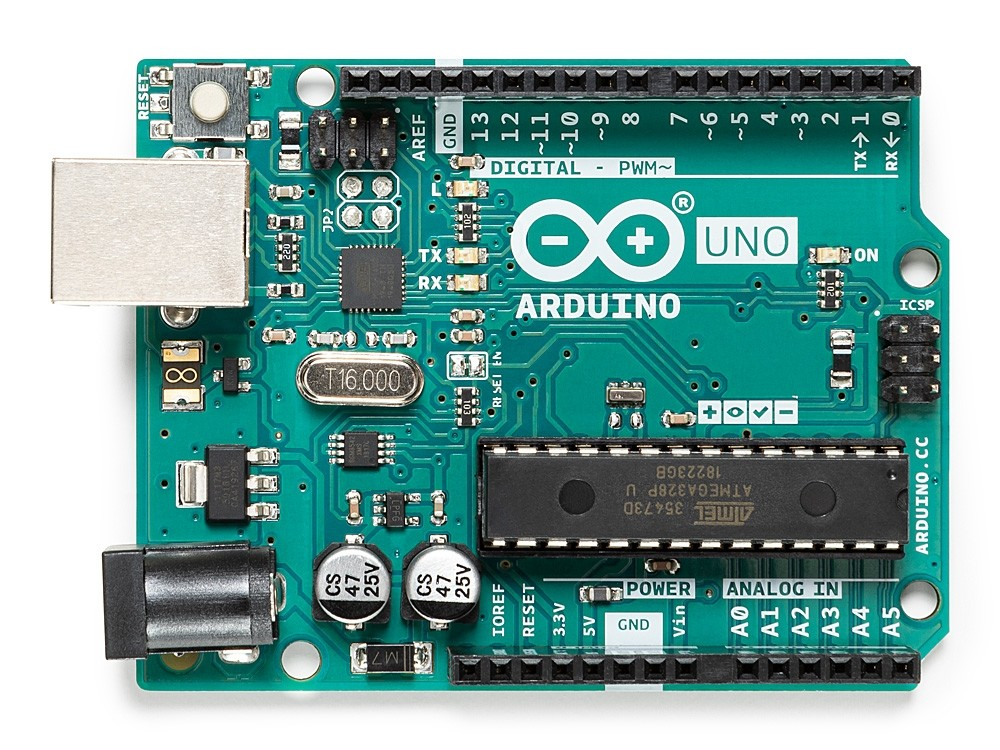
\includegraphics[width=0.3\textwidth]{Projets de conception/ArduinoUNO.jpg}
    \caption{La carte Arduino UNO rev3 où la puce principale (longue et noire vers le bas à droite) est le MCU \href{http://ww1.microchip.com/downloads/en/DeviceDoc/Atmel-7810-Automotive-Microcontrollers-ATmega328P_Datasheet.pdf}{ATmega328P} avec des \href{https://www.circuito.io/blog/arduino-uno-pinout/}{ entrées/sorties} situées le long en haut et en bas de la carte alors que l'alimentation et un port USB sont sur la gauche. Photo provenant du \href{https://store.arduino.cc/usa/}{magasin en ligne} de la compagnie Arduino.}
    \label{fig:ArduinoUNO}
\end{figure}

\subsubsection*{Qu'est qu'un Arduino peut faire?}
Cela dépend des périphériques disponibles sur le MCU utilisé, soit ATmega328P de Atmel pour la carte Arduino UNO. Quelques exemples sont de l’acquisition de données, de la synchronisation de signaux, du traitement de données en temps réel, etc. Parmi les périphériques du MCU que l’Arduino utilise, deux (au minimum) seront utiles à la conception du système:
\begin{itemize}
    \item le \href{https://en.wikipedia.org/wiki/Analog-to-digital_converter}{convertisseur analogique-numérique} (\textit{analog-to-digital converter}, ADC) qui permet de lire une tension analogique, par exemple aux bornes d’une photorésistance ou celle qui était fournie par une pomme de terre au début du cours(!),
    \item le générateur de signaux en   \href{https://en.wikipedia.org/wiki/Pulse-width_modulation}{modulation de largeur d'impulsions} (\textit{pulse-wave-modulation}, PWM) qui permet de contrôler certains composants qui ne nécessitent pas un courant élevé, par exemple la base d’un transistor.
\end{itemize}

 Pour utiliser ces fonctionnalités, Arduino a implémenté des fonctions simples à utiliser, soit les fonctions \texttt{AnalogRead}  et \texttt{DigitalWrite/AnalogWrite}. Afin de faire l’acquisition d’un signal via le schéma Tinkercad de l’Arduino, les entrées qui sont identifiées \textbf{ADC} ou encore \textbf{A0, A1, A2,} … devront être utilisées. Pour générer un signal, les sorties qui sont identifiées \textbf{PWM} seront utilisées. Arduino, voulant simplifier la tâche, a indiqué que certaines entrées étaient dédiées à des fonctions spécifiques, mais en réalité, c’est le MCU qui décide ce qui se passe sur une entrée et plusieurs fonctions différentes peuvent être utilisées sur une seule et même entrée.
 
\subsubsection*{Comment utiliser un Arduino?}
Il faut le programmer, sauf que les MCU n'acceptent pas directement des langages interprétés de haut niveau\footnote{Des librairies se développent cependant dans plusieurs langages tels Python (\href{https://github.com/tino/pyFirmata}{Firmata}, \href{https://pypi.org/project/pyserial/}{pyserial}, ...) et \href{https://www.mathworks.com/help/supportpkg/arduinoio/examples/getting-started-with-matlab-support-package-for-arduino-hardware.html}{MATLAB} pour communiquer avec une carte Arduino à partir d'un ordinateur ou encore être exécutées directement sur d'autres types de MCU avec \href{https://www.digikey.ca/en/maker/blogs/2018/python-on-hardware}{CircuitPython} par exemple.}. Le C et le C++ sont les langages majoritairement utilisés pour cette programmation puisqu’ils sont rapides d’exécution tout en étant relativement simples à coder pour des langages compilés. Heureusement, la compagnie Arduino offre une interface de programmation conviviale qui contient déjà plusieurs fonctions PRÉCODÉES (\href{https://www.arduino.cc/en/Tutorial/BuiltInExamples}{
didacticiels ici}) et Tinkercad offre même en parallèle une \href{https://scientiffic.medium.com/tinkercad-circuits-code-blocks-9953d47b5a3f}{programmation visuelle avec des briques Scratch} si désiré. 

\noindent Quelques conseils avant de se lancer dans la programmation Arduino:
\begin{itemize}
    \item Toutes les variables doivent toutes être déclarées au début, ainsi que leur \href{https://en.wikipedia.org/wiki/C_data_types}{type} avant de les utiliser ailleurs dans le code.
    \item La fonction \texttt{void functionName()~\{\}} signifie seulement que la fonction ne retourne rien, car il faut aussi déclarer ce que la fonction retourne. Si la fonction retourne un entier, il faut plutôt écrire \texttt{int functionName()~\{\}}.
    \item L’intégralité de ce qui se passe lorsque l’Arduino exécute se trouve dans la fonction \texttt{loop()~\{\}}.
    \item Le code dans la fonction \texttt{setup()~\{\}} ne sera exécuté qu’une fois au démarrage de l’Arduino.
    \item Le moniteur série dans Tinkercad permet de faire des actions équivalentes à la commande \texttt{print} rencontrée en Python et bien d'autres langages; cela pourrait simplifier la tâche.
\end{itemize}

\subsection*{Photorésistance}
Une photorésistance est un composant électrique dont la résistance varie en fonction de l'irradiance, c'est-à-dire l’intensité lumineuse mesurée en \si[inter-unit-product=\ensuremath{{}\cdot{}}]{\watt\per\meter\squared}. Ces photorésistances sont fabriquées à partir de matériaux semiconducteurs dont la conductivité augmente lorsqu’ils sont exposés à la lumière. Par conséquent, la résistance de celles-ci varie à l'inverse de l'irradiance. La Figure~\ref{fig:photoresistance} montre la représentation de la photorésistance dans l’environnement Tinkercad.

\begin{figure}[h]
    \centering
    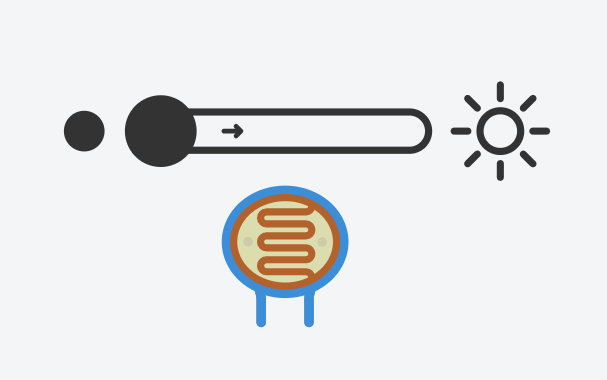
\includegraphics[width=0.4\textwidth]{Projets de conception/Photoresistance.png}
    \caption{Photorésistance dans l’environnement Tinkercad. La glissière au-dessus permet d’ajuster l’irradiance en démarrant la simulation, puis en sélectionnant la photorésistance. Dans le cadre de ce projet de conception, la période du jour est représentée par la position de l’indicateur sur la glissière, avec la position la plus à gauche représentant la nuit.}
    \label{fig:photoresistance}
\end{figure}

\subsection*{Conseils d'utilisation de transistor}
Finalement, le.s transistor.s peut.vent être utilisé.s dans la conception du circuit pour contrôler une charge (le moteur DC) qui serait placée entre le collecteur et l'émetteur et alimentée par une tension $V_{CE}$. Le mode interrupteur, donné en exemple à la Figure~\ref{fig:InterrupteurMoteur}, ou le mode amplificateur peut être utilisé. La tension de contrôle $V_{BE}$ peut être générée par la carte Arduino UNO, ce qui permettrait d’adapter l’alimentation du moteur en fonction de la résistance d’une photorésistance qui pourra également être lue par l’Arduino.

%Refaire ce circuit avec des transistors à jonction bipolaire pour avoir une image avec RPM corrects. 
\begin{figure}[h]
    \centering
    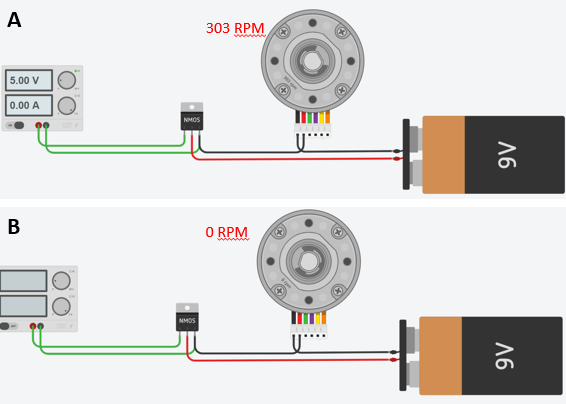
\includegraphics[width=0.35\textwidth]{Projets de conception/InterrupteurMoteur.png}
    \caption{Moteur DC~437~RPM actionné en (A) puis éteint en (B) avec le transistor qui joue le rôle d'interrupteur. (A) Avec une tension de suffisante entre la base et l'émetteur du transistor, l’interrupteur est fermé et le courant circule entre la batterie de \SI{9}{\volt} et le moteur DC. (B) La base du transistor n'est plus sous tension et l'interrupteur est ouvert, d'où aucun courant ne circule dans le moteur.}
    \label{fig:InterrupteurMoteur}
\end{figure}

\end{document}
